% mainfile: ../../../../master.tex
\subsection{RNA quantification with Qubit\texttrademark ~RNA Assay Kit}
% The part of the label after the colon must match the file name. Otherwise,
% conditional compilation based on task labels does NOT work.
\label{task:20180113_cj2}
\tags{rna,qnt,lab}
\authors{cj}
%\files{}
%\persons{}

\begin{figure}[H]
    \centering
    \caption{Illustration for the Qubit\texttrademark ~RNA assay}
    \label{fig:20180113_rna_qubit}
    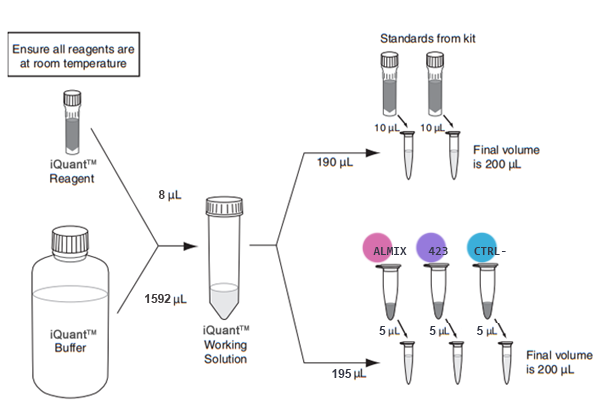
\includegraphics[width=0.7\textwidth]{graphics/schemas/20180113_rna_qubit.png}
\end{figure}

\mistake{I was unable to calibrate the Qubit\texttrademark, so I used the old calibration to obtain results.}

The Qubit\texttrademark ~RNA Assay Kit contains two standards: \#1 and \#2. But for some reasons, there are four different tubes for standard \#2. Last time I used this kit, I had trouble calibrating the Qubit\texttrademark and I ended up testing all four standard \#2. This time, to avoid spending time making several working solution, I decide to prepare the assay considering I might have to use the four different standards \#2. This is the reason why I prepare my assay for 8 samples (even though it's not shown clearly in figure \ref{fig:20180113_rna_qubit}): 3 samples + 1 STD\#1 + 4 STD\#2. Unfortunately, I was unable to calibrate the Qubit\texttrademark even after several trials with all different standard \#2. Finally, I gave up on the calibration and used the previous calibration (which I believe was done by me on the 4\textsuperscript{th} January 2018).

I resuspended the RNA pellet in 50~\uL of 10~mM Tris-HCl buffer. Then I used 2~\uL for the Nanodrop analysis, and 5~\uL for the Qubit analysis which means that the final volume is 43~\uL. 

The concentrations of RNA and the calculated quantities of RNA are summarised in table \ref{tab:20180113_nuc_acid_qnt}.

\begin{table}[H]
\caption{Total RNA quantities in samples measured with Qubit\texttrademark ~RNA HS Assay Kit}
\label{tab:20180113_nuc_acid_qnt}
\centering
\begin{tabular}{l r r r r}
\toprule
Sample ID & \textmu g/mL & $V_f$ (mL) & m (\textmu g) & m (ng) \\ \midrule
\texttt{CJ20180103\_RNA\_ALMIX} & 38.00 & 0.043 & 1.634 & 1634 \\
\texttt{CJ20180103\_RNA\_423} & 17.70 & 0.043 & 0.602 & ~602 \\
\texttt{CJ20180103\_RNA\_CTRL} & TOO LOW & 0.043 & NA & ~~NA \\
\bottomrule
\end{tabular}
\end{table}
 